\documentclass{article}[18pt]
\ProvidesPackage{format}
%Page setup
\usepackage[utf8]{inputenc}
\usepackage[margin=0.7in]{geometry}
\usepackage{parselines} 
\usepackage[english]{babel}
\usepackage{fancyhdr}
\usepackage{titlesec}
\hyphenpenalty=10000

\pagestyle{fancy}
\fancyhf{}
\rhead{Sam Robbins}
\rfoot{Page \thepage}

%Characters
\usepackage{amsmath}
\usepackage{amssymb}
\usepackage{gensymb}
\newcommand{\R}{\mathbb{R}}

%Diagrams
\usepackage{pgfplots}
\usepackage{graphicx}
\usepackage{tabularx}
\usepackage{relsize}
\pgfplotsset{width=10cm,compat=1.9}
\usepackage{float}

%Length Setting
\titlespacing\section{0pt}{14pt plus 4pt minus 2pt}{0pt plus 2pt minus 2pt}
\newlength\tindent
\setlength{\tindent}{\parindent}
\setlength{\parindent}{0pt}
\renewcommand{\indent}{\hspace*{\tindent}}

%Programming Font
\usepackage{courier}
\usepackage{listings}
\usepackage{pxfonts}

%Lists
\usepackage{enumerate}
\usepackage{enumitem}

% Networks Macro
\usepackage{tikz}


% Commands for files converted using pandoc
\providecommand{\tightlist}{%
	\setlength{\itemsep}{0pt}\setlength{\parskip}{0pt}}
\usepackage{hyperref}

% Get nice commands for floor and ceil
\usepackage{mathtools}
\DeclarePairedDelimiter{\ceil}{\lceil}{\rceil}
\DeclarePairedDelimiter{\floor}{\lfloor}{\rfloor}

% Allow itemize to go up to 20 levels deep (just change the number if you need more you madman)
\usepackage{enumitem}
\setlistdepth{20}
\renewlist{itemize}{itemize}{20}

% initially, use dots for all levels
\setlist[itemize]{label=$\cdot$}

% customize the first 3 levels
\setlist[itemize,1]{label=\textbullet}
\setlist[itemize,2]{label=--}
\setlist[itemize,3]{label=*}

% Definition and Important Stuff
% Important stuff
\usepackage[framemethod=TikZ]{mdframed}

\newcounter{theo}[section]\setcounter{theo}{0}
\renewcommand{\thetheo}{\arabic{section}.\arabic{theo}}
\newenvironment{important}[1][]{%
	\refstepcounter{theo}%
	\ifstrempty{#1}%
	{\mdfsetup{%
			frametitle={%
				\tikz[baseline=(current bounding box.east),outer sep=0pt]
				\node[anchor=east,rectangle,fill=red!50]
				{\strut Important};}}
	}%
	{\mdfsetup{%
			frametitle={%
				\tikz[baseline=(current bounding box.east),outer sep=0pt]
				\node[anchor=east,rectangle,fill=red!50]
				{\strut Important:~#1};}}%
	}%
	\mdfsetup{innertopmargin=10pt,linecolor=red!50,%
		linewidth=2pt,topline=true,%
		frametitleaboveskip=\dimexpr-\ht\strutbox\relax
	}
	\begin{mdframed}[]\relax%
		\centering
		}{\end{mdframed}}



\newcounter{lem}[section]\setcounter{lem}{0}
\renewcommand{\thelem}{\arabic{section}.\arabic{lem}}
\newenvironment{defin}[1][]{%
	\refstepcounter{lem}%
	\ifstrempty{#1}%
	{\mdfsetup{%
			frametitle={%
				\tikz[baseline=(current bounding box.east),outer sep=0pt]
				\node[anchor=east,rectangle,fill=blue!20]
				{\strut Definition};}}
	}%
	{\mdfsetup{%
			frametitle={%
				\tikz[baseline=(current bounding box.east),outer sep=0pt]
				\node[anchor=east,rectangle,fill=blue!20]
				{\strut Definition:~#1};}}%
	}%
	\mdfsetup{innertopmargin=10pt,linecolor=blue!20,%
		linewidth=2pt,topline=true,%
		frametitleaboveskip=\dimexpr-\ht\strutbox\relax
	}
	\begin{mdframed}[]\relax%
		\centering
		}{\end{mdframed}}
\lhead{Networks and Systems - Networks}


\begin{document}
\begin{center}
\underline{\huge Data Link Layer}
\end{center}
\section{Frames}
\begin{itemize}
	\item Link layer accepts packets from the network layer, and encapsulates them into frames that it sends using the physical layer; reception is the opposite process
	\item The physical layer (below) is responsible for the transmission of raw sequences of bits
\end{itemize}
\begin{center}
	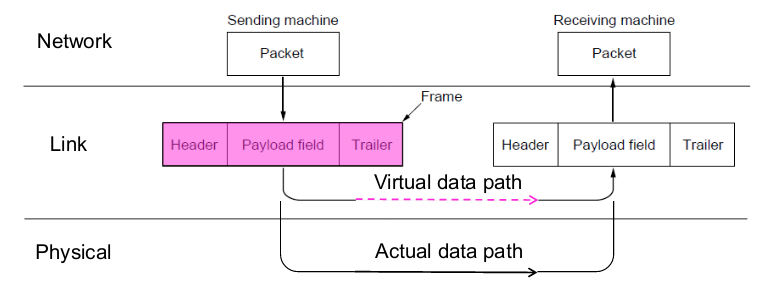
\includegraphics[scale=0.7]{frame}
\end{center}
\section{Framing methods}
\subsection{Byte count}
Frame begins with a count of the number of bytes in it - simple, but difficult to resynchronize after an error. If any of the counts are incorrect then everything will be shifted wrong and all the frames will be incorrect.
\subsection{Headers and trailers}
We add a header (e.g. the length of the data, etc.) and a trailer (extra data that can be used e.g. error-detection or error-correction)
\begin{center}
	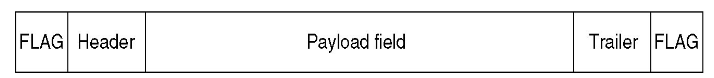
\includegraphics[scale=0.7]{flag}
\end{center}
Two adjacent frames are separated by a flag
\subsection{Byte stuffing}
Special flag bytes delimit frames; occurrences of flags in the data must (escapes) - longer, but easy to resynchronize after error\\
\\
If the flag value is found in the data you get lost again. The solution to this is byte or bit stuffing
\begin{center}
	\includegraphics[scale=0.7]{"byte stuffing"}
\end{center}
\begin{center}
	\includegraphics[scale=0.7]{"byte stuffing1"}
\end{center}
This is the same idea as doing $\backslash$delta in latex
\subsection{Bit stuffing}
\begin{center}
	\includegraphics[scale=0.7]{"bit stuffing"}
\end{center}
This is useful where you aren't working in bytes, as frames can be any size now\\
\\
The flag is six consecutive ones. Within the data, a zero is stuffed after each five consecutive ones to void instances of the flag in the data\\
Bit stuffing
\begin{enumerate}[label=(\alph*)]
	\item The original data
	\item The data as they appear on the line
	\item The data as they are stored in receiver's memory after de-stuffing
\end{enumerate}
Sender:
\begin{itemize}
	\item Encloses packet (bit stream): 0 1 1 1 1 1 0
	\item Appends a 0 after each 1 1 1 1 1 in body (bit stuffing)
\end{itemize}
Receiver, upon receiving 0 1 1 1 1 1:
\begin{itemize}
	\item next bit 0: stuffed bit is removed
	\item next bit 1
	\begin{itemize}
		\item if next bit 0: end of frame marker
		\item if next bit 1: error
	\end{itemize}
\end{itemize}
\section{Error detection and correction}
\begin{itemize}
	\item Errors occur during frame transmission
	\item Two strategies to deal with error
	\begin{itemize}
		\item Include enough redundant information to help receivers deduce original data (\textbf{error correcting})
		\item Include enough information to deduce an error occurred (\textbf{error detecting})
		\item Neither error-correcting codes nor error-detecting codes can handle all possible errors
	\end{itemize}
\end{itemize}
\textbf{EDC} = Error detection and correction bits (redundancy)\\
\textbf{D} = Data protected by error checking, may include header fields\\
\\
Error detection is not 100\% reliable, protocol may miss some errors, but rarely
\begin{center}
	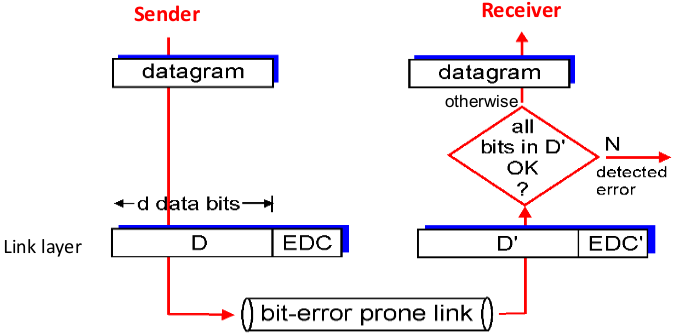
\includegraphics[scale=0.7]{EDC}
\end{center}
\section{Codeword}
\begin{defin}[Codeword]
The message with check bits added	
\end{defin}
\begin{itemize}
	\item A frame consists of m data (message) bits and r redundant (check) bits
	\item n-bit codewords with n=m+r
\end{itemize}
\newpage
\section{Error codes}
Error codes add structured redundancy to data so errors can be either detected, or corrected

\subsection{Hamming codes}
\begin{defin}[Hamming distance]
The number of bit positions in which two codewords differ
\end{defin}
We will see a specific hamming code that corrects a single error:
\begin{itemize}
	\item \textbf{Encoding}: we number the data bits starting from one and skipping the powers of two. The powers of two are reserved for parity bits, the rest are message bits.
	\item \textbf{Decoding}: calculate all parities. If they are all OK, there was no error. If not, add up the positions of the incorrect ones - this gives us the position of the error
\end{itemize}
Hamming code gives a simple way to add check bits and correct up to a single bit error
\begin{itemize}
	\item Check bits are parity over subsets of the codeword
	\item Recomputing the parity sums (syndrome) gives the position of the error to flip, or 0 if there is no error
\end{itemize}
\section{Error detection}
\subsection{Parity}
Parity bit is added as the modulo 2 sum of data bits\\
\\
\textbf{Single bit parity} - detect single bit errors - this has one parity bit for whatever the length of the message\\
\\
\textbf{Two dimensional bit parity} - detect and correct single bit errors
\begin{itemize}
	\item Write the message in rows
	\item Calculate the parity bit for both the row and column
	\item These can then be used to correct a bit error as there will be a parity error on the corresponding row and column of the bit
\end{itemize}


\subsection{Checksum}
The sender:
\begin{enumerate}
	\item Data is divided into k segment each of m bits (normally 16 bit integers) and summed
	\item The 1s complement of the sum forms the checksum.
	\item The checksum segment is sent along with the data segments
\end{enumerate}
The receiver
\begin{enumerate}
	\item All received segments are added
	\item The sum is complemented
	\item If the result is zero, the received data is OK; otherwise wrong
\end{enumerate}
\subsection{Cyclic Redundancy Check}
This is a more advanced technique, which uses manipulations with polynomials. This is one of the most commonly used error detection codes\\
\\
Basic approach:
\begin{itemize}
	\item Let M1 be the message of n-bits
	\item M1 is padded with CRC code and send it
	\item CRC is generated using a given polynomial P1 (or divisor)
	\item P1 is agreed between sender and receiver
	\item Receiver gets M1 + CRC and extracts the M1 using P1
\end{itemize}
\begin{center}
	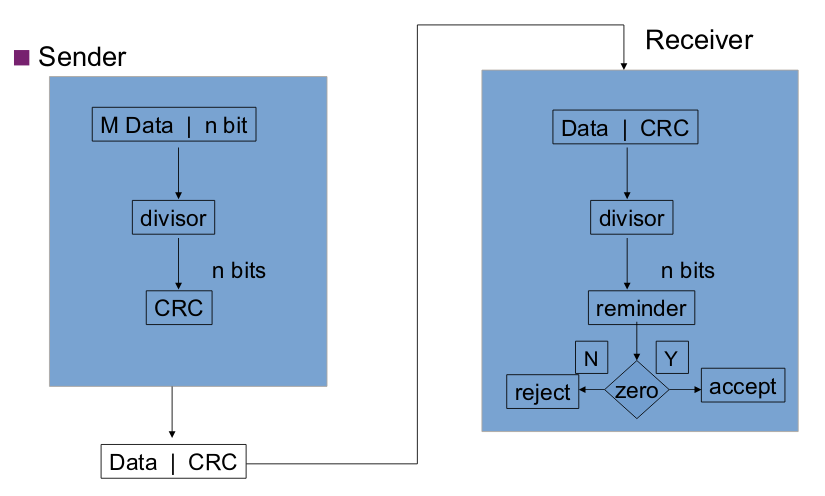
\includegraphics[scale=0.7]{CRC}
\end{center}

\end{document}